
\FloatBarrier
\section{Система Лоренца} % _LOR_

\LinkRef{
  lor: ASAU-22, 23, 24, 25, 26.
  % ~/doc/tex/asau/asau22/atu/atu.tex
  % ~/doc/tex/asau/asau23/atu/atu.tex
  % ~/doc/tex/asau/asau24/atu/atu.tex
  APIR-2012. CSIT-2015. ISDMCI-2014, ISDMCI-2015.
  ITMM-2012, ITMM-2014, ITMM-2015, DSMP-2016
}


В качестве первой идентифицируемой хаотической системы рассмотрим классическую
систему Лоренца, динамика которой описывается системой
уравнений~\cite{moon_chaotic_vibr,anisch_nonlin_eff,chulichkcov_mm_ml_dyn}:
%
\begin{equation}
\begin{cases}
  \dot{x} = \sigma (y-x ) , \\
  \dot{y} = x (r-z) - y , \\
  \dot{z} = x y - b z .
\end{cases}
\label{atu:eq:lor}
\end{equation}

Наиболее ценным с точки зрения идентификации является параметр
$r$, определяющий как энергетическое состояние системы,
так и вид динамики системы.
Это подтверждают
расмотренные в дальнейшем физические обосноснования.
Для определённости зададим остальные параметры следующим классическим образом:
$b = 2.6666667$, $\sigma = 10$, если не будет явно указано обратное.


При малых значениях параметра $r$ система демонстрирует
затухающие колебания (рис.~\ref{atu:f:lor_attractor_fading}).

\begin{figure}[h!]
\begin{center}
  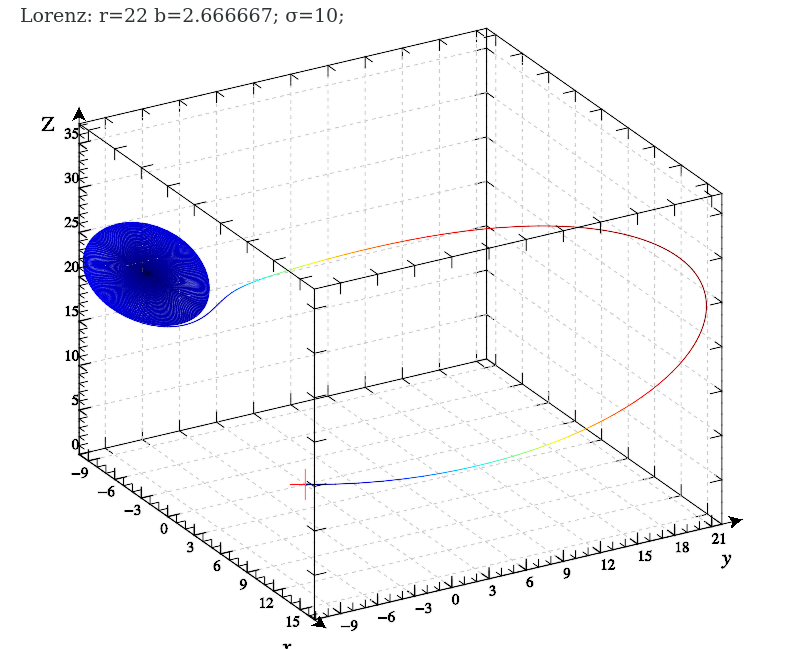
\includegraphics[width=0.49\textwidth]{p/cha/lor/lor0-p_xyz_r=022.png}
  \hfill
  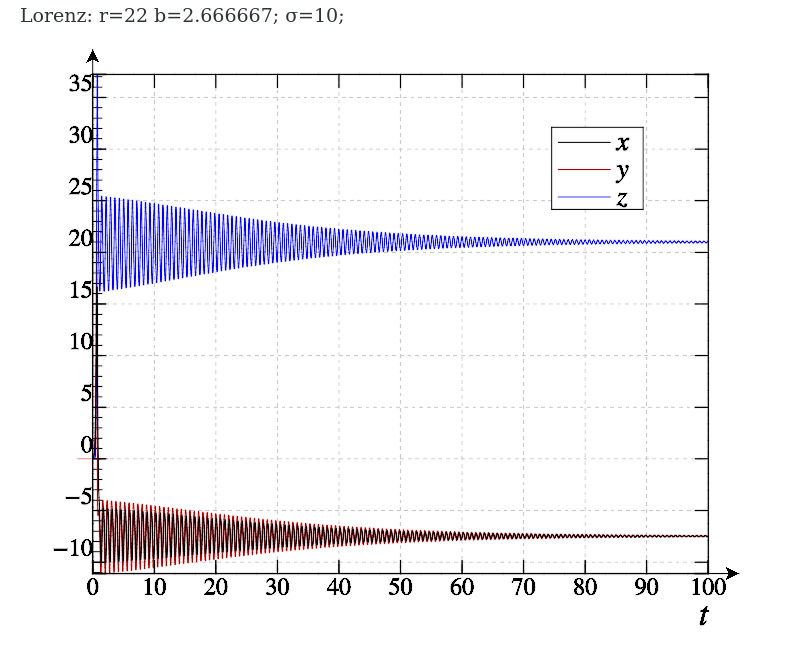
\includegraphics[width=0.49\textwidth]{p/cha/lor/lor0-p_t_r=022.png}
\end{center}
  \caption{Аттрактор и поведение переменных состояния системы Лоренца (\ref{atu:eq:lor}) в режиме затухающих колебаний ($r=22$)}
\label{atu:f:lor_attractor_fading}
\end{figure}

Далее,  в широком диапазоне значения параметра $r$
система проявляет хаотическую динамику. Помимо
этого, спектр данной системы в хаотическом режиме довольно широк
(рис.~\ref{atu:f:lor_attractor_phase_chaos28})
и не имеет доминирующих частот, что не характерно для многих систем
динамического хаоса.

\begin{figure}[h!]
\begin{center}
  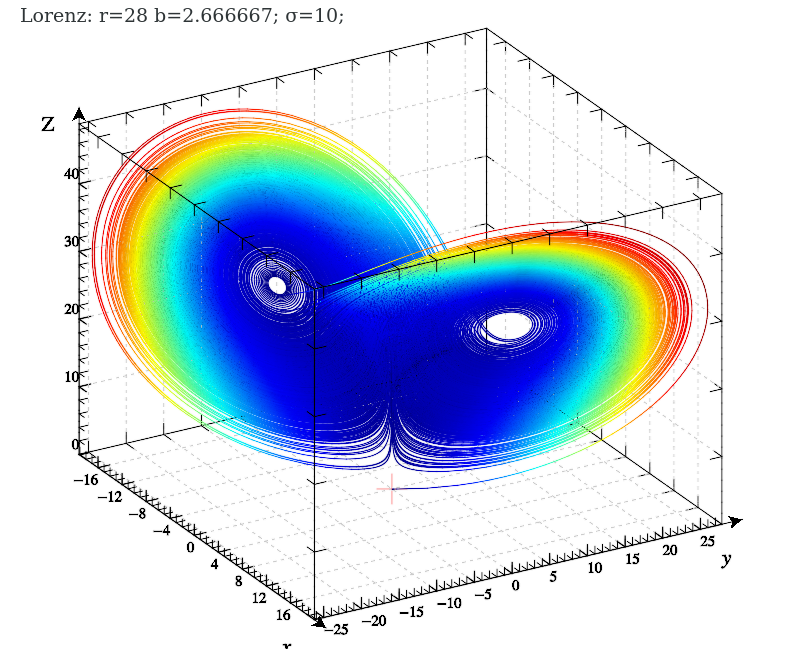
\includegraphics[width=0.49\textwidth]{p/cha/lor/lor0-p_xyz_r=028.png}
  \hfill
  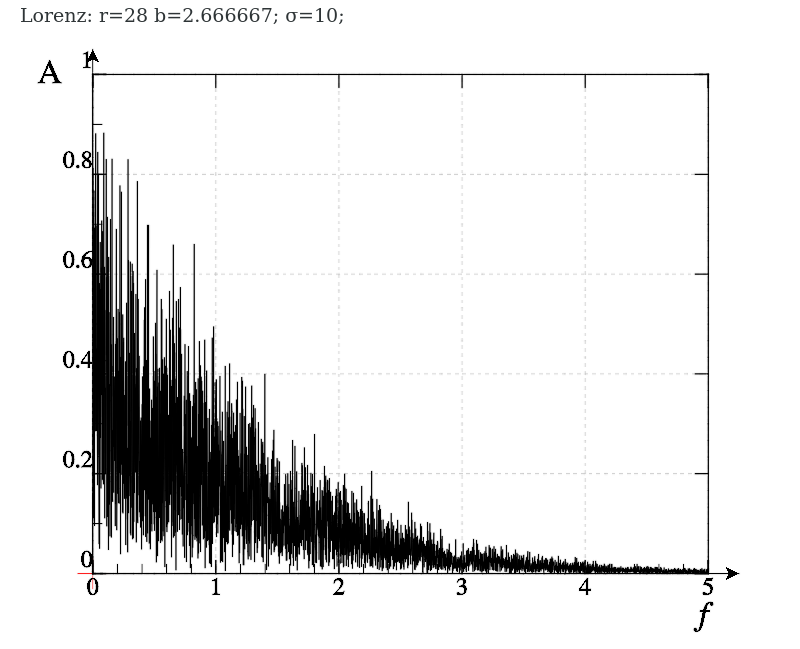
\includegraphics[width=0.49\textwidth]{p/cha/lor/lor0_fft-p_f_r=028.png}
\end{center}
  \caption{Аттрактор и спектр системы Лоренца (\ref{atu:eq:lor}) в хаотическом режиме ($r=28$)}
\label{atu:f:lor_attractor_phase_chaos28}
\end{figure}

При дальнейшем росте параметра $r$ динамика системы становится
сложно-периодической, с явно выраженным линейчатым спектром
(рис.~\ref{atu:f:lor_attractor_phase_200})

\begin{figure}[h!]
\begin{center}
  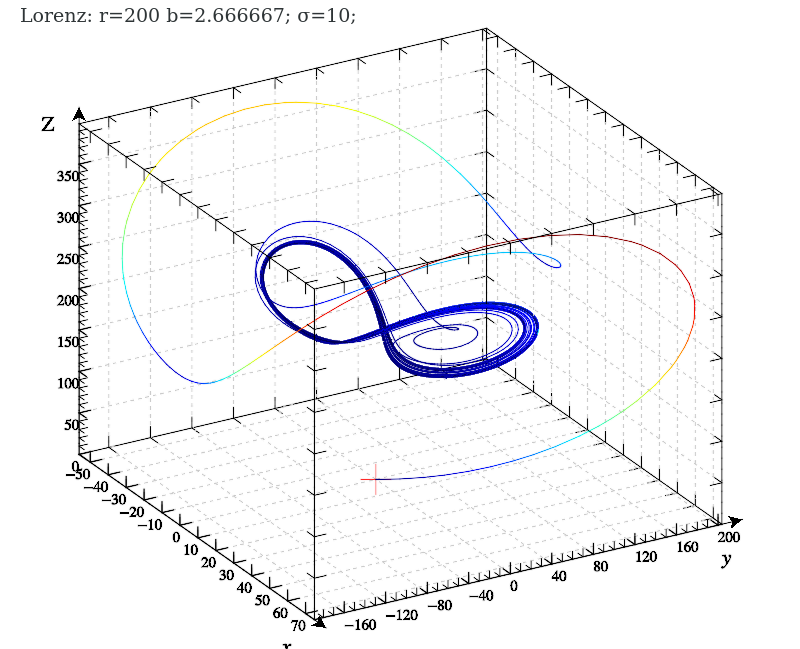
\includegraphics[width=0.49\textwidth]{p/cha/lor/lor0-p_xyz_r=200.png}
  \hfill
  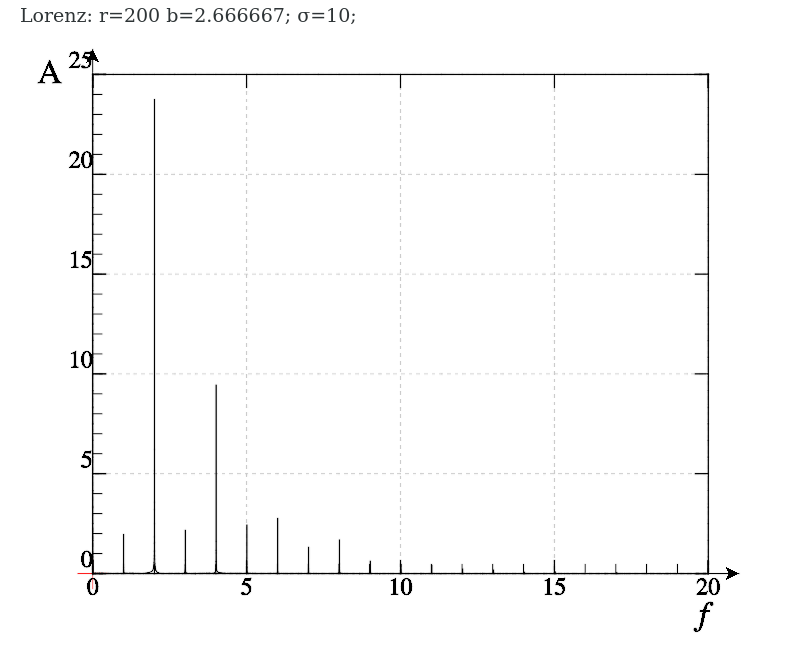
\includegraphics[width=0.49\textwidth]{p/cha/lor/lor0_fft-p_f_r=200.png}
\end{center}
  \caption{Аттрактор и спектр системы Лоренца (\ref{atu:eq:lor}) в сложно-периодическом режиме ($r=200$)}
\label{atu:f:lor_attractor_phase_200}
\end{figure}



Динамическая система Лоренца является одной из наиболее изученных
хаотических систем~\cite{neimark_stoch_chaos_vibro}.
При этом, существует множество физических систем, для
описания которых применима модель Лоренца. Это дает определённые основания
предполагать, что синтез критерия идентификации, основанного на физических
принципах, для данной системы будет успешным.


Для синтеза критерия идентификации параметра $r$ системы (\ref{atu:eq:lor}), рассмотрим
набор физических систем, для моделирования которых применяется система
Лоренца.

Исторически первой такой системой, рассмотренной самим Лоренцом, является
задача о тепловой конвекции жидкости в плоском слое. Исходная система
уравнений гидродинамики имеет вид:
%
%
\begin{equation}
\begin{cases}
  \pd{\vec{v}}{t} + ( \vec{v} \nabla ) \vec{v} = - \frac{\nabla p}{\rho} + \nu \Delta \vec{v} + \vec{g}, \\
  \pd{\rho}{t} + \nabla ( \rho \vec{v} ) = 0 , \\
  \pd{T}{t} +\nabla ( T \vec{v} ) = \chi \Delta T , \\
  \rho = \rho_0 \left( 1 - \gamma (T - T_0) \right) .
\end{cases}
\label{atu:eq:lor_gidro}
\end{equation}
%
где
$\vec{v} $   -- поле скоростей,
$T$ -- поле температуры,
$T_0$ и $T_0+\Delta T$   -- температуры на верхней и нижней границе соответственно,
$\rho$ и $p$ -- поля плотности и давления,
$g$ -- ускорение свободного падения,
$\nu$, $\chi$, $\gamma$  -- коэффициенты кинематической вязкости, температуропроводности и
теплового расширения соответственно.

При приближении системы (\ref{atu:eq:lor_gidro}) к виду (\ref{atu:eq:lor}),
переменные и параметры системы
Лоренца определяются следующим образом: $x$ задаёт скорость вращения валов
течения, $y$, $z$ -- соответствуют распределению температуры по горизонтали и
вертикали.
$\sigma$   -- число Прандтля (отношение коэффициентов кинематической вязкости и
температуропроводности). Параметр $b$ определяет отношения размеров ячейки.
$r$ -- (идентифицируемый параметр) -- приведённое число Релея, определяющее
энергетические параметры конвекционного течения.

Из трёх переменных состояния проще всего наблюдению поддаётся переменная
$x$. С другой стороны, так как параметр $r$ определяет энергетические
соотношения в системе, то и критерий качества должен представлять собой
квадратичную форму от $x$, причём усреднённую на интервале времени,
существенно большем, чем характерное время оборота жидкостного вала.

Другой системой, для моделирования которой применяется система Лоренца --
это модель одномодового лазера. В этой модели переменной $x$ соответствует
амплитуда поля в резонаторе, $y$ -- поляризации, $z$ -- инверсии заселённости
квантовых уровней активной среды. Параметры $\sigma$ и $b$
определяются отношениями коэффициентов релаксации, а искомый параметр $r$
определяется удельной мощностью накачки.

Как и в случае гидродинамической системы, наиболее просто наблюдаемым
параметром является $x$ -- именно он определяет выходную интенсивность. И
опять же, по аналогии -- идентифицируемый параметр $r$ определяет энергетику
системы. При переходе от амплитуды к мощности совершенно аналогично
следует использовать квадратичную зависимость.

Также система (\ref{atu:eq:lor}) применима для
моделирования конвекции жидкости в замкнутом подогреваемом петле,
динамики водяного колеса, осцилляторе с трением и других~\cite{kuznetsov_dyn_chaos}.

Таким образом, в первую очередь следует проверить применимость
критерия вида $q_{x^2}$. Тем не менее, проверим все
критерии данного вида, применимые к данной системе.
На рис.~\ref{atu:f:lor_q} приведены исследуемые зависимости
$q_{*}(r)$, полученные путём моделирования динамики
системы \ref{atu:eq:lor} для различных значений параметра~$r$,
при усреднении на значительном временном интервале $\tau_q=500$.


\begin{figure}[h!]
  \centerline{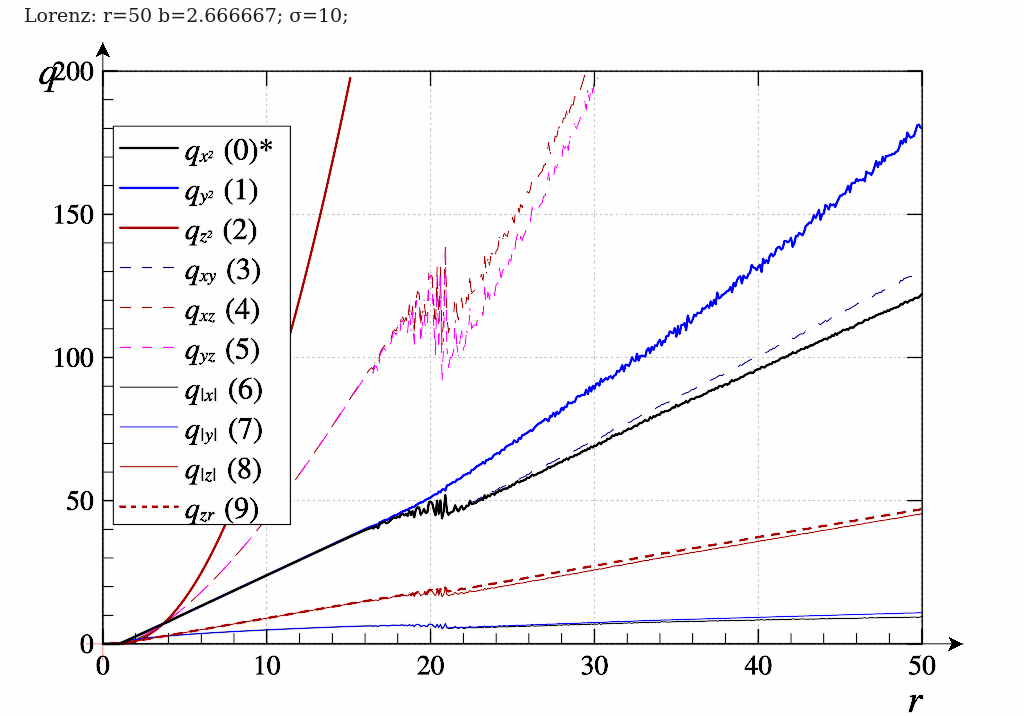
\includegraphics[width=0.7\textwidth]{p/cha/lor/lor_q-p_q_r.png} }
  \caption{Рассматриваемые критерии для системы Лоренца}
  \label{atu:f:lor_q}
\end{figure}

Анализ графиков позволяет сделать вывод, что практически все
рассмотренные виды критериев должны позволять построить
работоспособную систему идентификации. При этом,
большая часть графиков, в том числе и изначально
предложенный $q_{x^2}$, теряют монотонность
при переходе от режима затухающих колебаний к хаотическому,
что может помешать процессу идентификации вблизи этой точки.
Тем не менее, режим затухающих колебаний не представляет
практического интереса, и этим недостатком можно пренебречь.
Этого недостатка лишён критерий $q_{y^2}$, однако,
в рассматриваемых физических задачах значение
$y(t)$ наблюдать сложнее. К тому же, в первом приближении
зависимость $q_{x^2}(r)$ -- линейная, а
$q_{y^2}(r) \sim \sqrt{r}$.
Спектры же сигналов $x(t)$, $y(t)$ и $z(t)$
имеют практически одинаковую структуру.
Поэтому, в дальнейших исследованиях ограничимся
критериями
$q_{x^2}$ и
$q_{y^2}^2$.

Следующая зависимость, необходимая для синтеза
системы идентификации -- $ \sigma_q(\tau_q) $
или же  $ \sigma_q(a_q) $ -- соотношение между
временем оценивания $\tau_q$ и среднеквадратичной
ошибкой измерения критерия.
Для моделирования непосредственных погрешностей измерения величин
$x(t)$ и $y(t)$ использовался шум с нормальным распределением
и параметрами $\sigma_w=0.5$ и $\tau_w=0.05$.
Для оценивания требуемой зависимости, для каждого
значения $\tau_q$ из заданного диапазона
проводилось $N=200$ процессов моделирования динамики системы,
и в случайный момент (достаточно далеко отстоящий от точки $t=0$ для исключения краевых эффектов)
проводилось измерение и запоминание выбранного критерия.
При этом, для усреднения величины $q$ использовалось 2 метода:
простейший линейный, вида (\ref{atu:eq:qlin}), и скользящее среднее.
Полученные зависимости, обозначенные соответственно
$\sigma_{ql}$ и $\sigma_{qa}$, представлены на
рис.~\ref{atu:f:lor_qy2_tau} и~\ref{atu:f:lor_qx2_tau}.


\begin{figure}[h!]
\begin{center}
  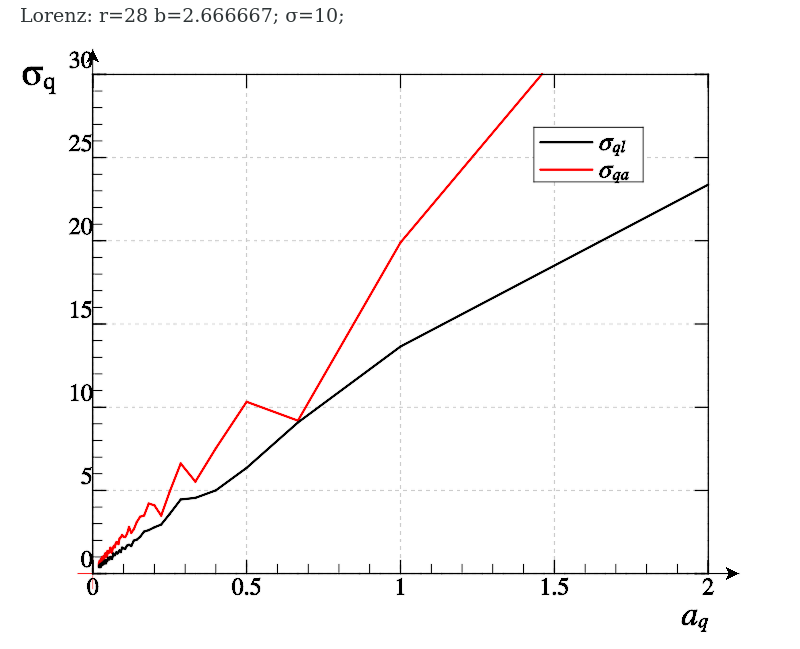
\includegraphics[width=0.49\textwidth]{p/cha/lor/lor_q_tau-p_aq_sd.png}
  \hfill
  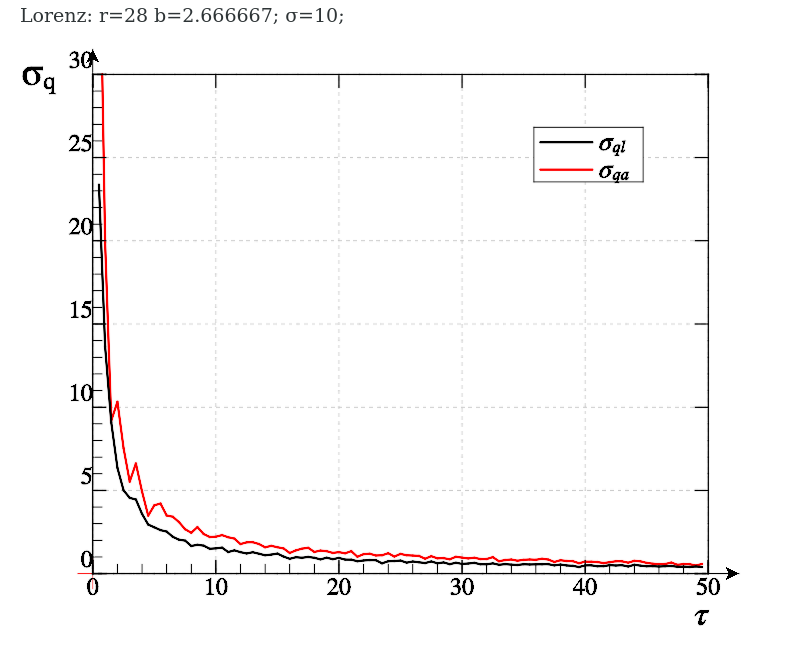
\includegraphics[width=0.49\textwidth]{p/cha/lor/lor_q_tau-p_tau_sd.png}
\end{center}
  \caption{Зависимости $\sigma_{q}(a_q)$ и $\sigma_{q}(\tau_q)$ для системы Лоренца, критерий  $q_{y^2}$}
\label{atu:f:lor_qy2_tau}
\end{figure}


\begin{figure}[h!]
\begin{center}
  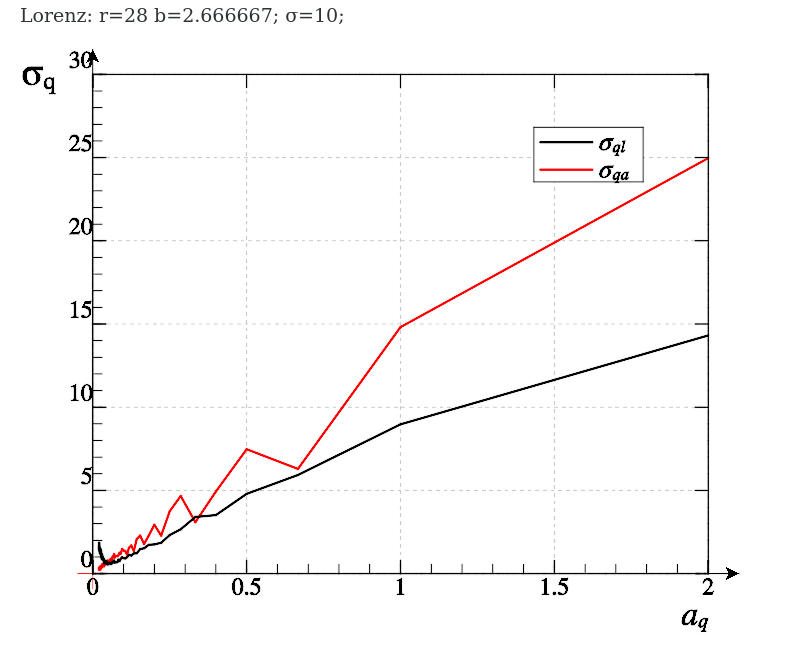
\includegraphics[width=0.49\textwidth]{p/cha/lor/lor_qx2_tau-p_aq_sd.png}
  \hfill
  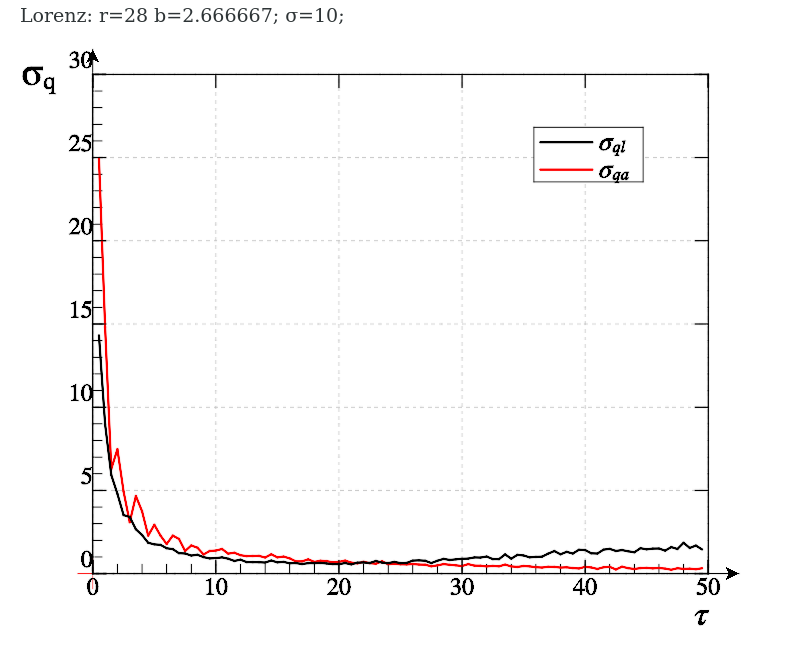
\includegraphics[width=0.49\textwidth]{p/cha/lor/lor_qx2_tau-p_tau_sd.png}
\end{center}
  \caption{Зависимости $\sigma_{q}(a_q)$ и $\sigma_{q}(\tau_q)$ для системы Лоренца, критерий $q_{x^2}$}
\label{atu:f:lor_qx2_tau}
\end{figure}

Анализ полученных зависимостей позволяет сделать
несколько выводов. Прежде всего, для рассматриваемой системы
результат усреднения с помощью значительно более затратного
в реализации метода скользящего среднего практически везде
уступает более простому методу. Таким образом,
при реализации методов идентификации в условиях с ограниченным ресурсами,
например на микроконтроллерной платформе в реальном времени,
нет смысла реализовывать ресурсоёмкоё скользящее среднее.
Далее, сам вид зависимости оказался достаточно простым:




\begin{figure}[h!]
  \centerline{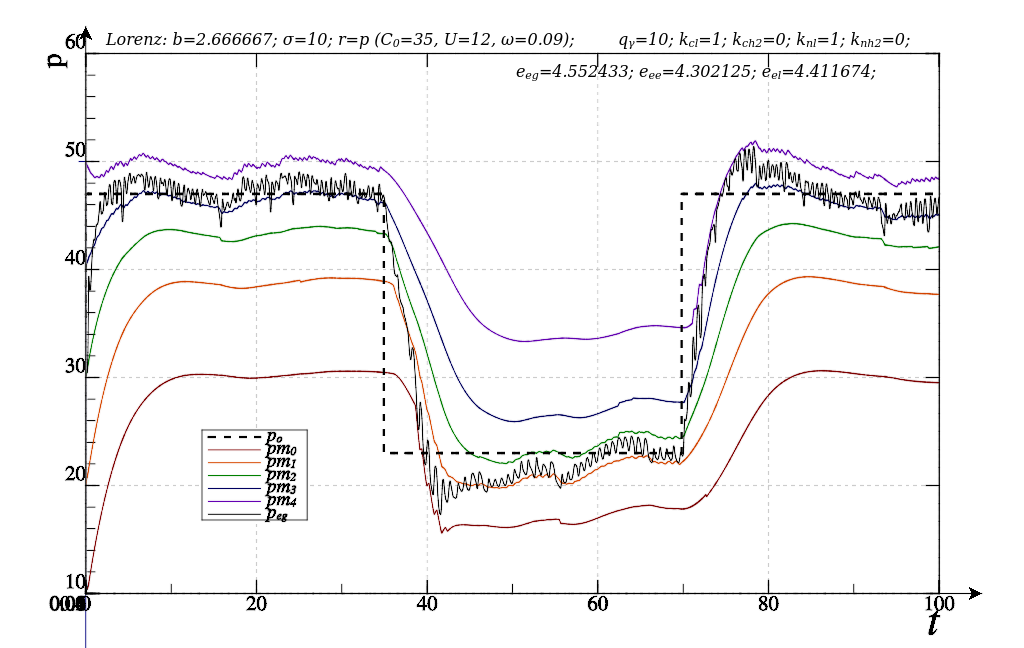
\includegraphics[width=0.7\textwidth]{p/cha/lor/lor_m5pf-pl_n_sign.png} }
  \caption{Процесс идентификации параметра ``$r$'' системы Лоренца}
  \label{atu:f:lor_id_mp5_sign}
\end{figure}

\[
  r_o(t) = p_o(t) = p_0 +  U_{p} \sign \sin( \omega_{p} t ),
\]


\begin{figure}[h!]
  \centerline{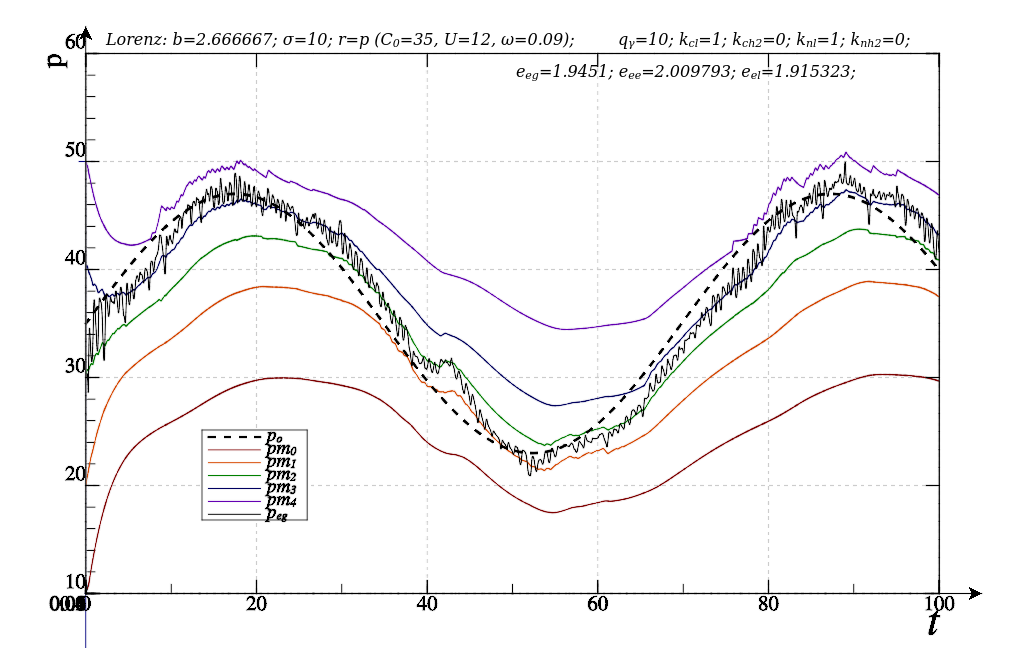
\includegraphics[width=0.7\textwidth]{p/cha/lor/lor_m5pf-pl_n_sin.png} }
  \caption{Процесс идентификации параметра ``$r$'' системы Лоренца}
  \label{atu:f:lor_id_mp5_sin}
\end{figure}

\[
  r_o(t) = p_o(t) = p_0 +  U_{p} \sin( \omega_{p} t ),
\]


% habr: 
% 1. Конвекция в тороидальной трубе (Ланда П.С. Нелинейные колебания и волны. — М: Либроком, 2010, с. 454-455)
% 2. Одномодовый лазер (Покровский Л.А. Решение системы уравнений Лоренца в
%  асимптотическом пределе большого числа Релея. I. Система Лоренца в простейшей
%  квантовой модели лазера и приложение к ней метода усреднения // Теоретическая
%  и математическая физика, 1985, т. 62, №2, с. 272-290);
% 3. Осциллятор с инерционным возбуждением (Неймарк Ю.И., Ланда П.С.
% Стохастические и хаотические колебания. — М: Либроком, 2009, с. 288-295).
